% !TEX root = ../thesis-example.tex
%
\chapter{From mobility patterns to scaling}
\label{sec:from_mobility_patterns_to_scaling}


In particular, we show that the dependence on population size of the total
number of miles driven daily, the total length of the road network, the total
traffic delay, the total consumption of gasoline, the quantity of $CO_2$ emitted
and the relation between area and population of cities, are all governed by a
single parameter which characterizes the sensitivity to congestion. 


The recent availability of an unprecedented amount of data has made possible
quantitative studies of cities~\cite{Fujita:1999,Batty:2007,Marshall:2004},
opening the way to a Science of Cities. In particular, the discovery of
allometric scaling relationships in cities has driven the quantitative research
on urban systems in the past years. Indeed, there is a great amount of evidence
to show that different socio-economic indicators in cities, such as the GDP, the
crime rate, the number of patents as well as different structural indicators
such as the total length of the road network, the urbanized land area, etc.,
exhibit robust scaling relationships with respect to
population~\cite{Newman:1989,Makse:1995,Pumain:2006,Bettencourt:2007,Samaniego:2008,Rozenfeld:2008,Pan:2013}.
The existence of these simple scaling relationship hints at the existence of
universal processes shared by urban systems, and thus at the possibility of
modeling cities.\\

A common trait shared by all complex systems --including cities-- is the
existence of a large variety of processes occuring over a wide range of time and
spatial scales. The main obstacle to the understanding of these systems
therefore resides in uncovering the hierarchy of processes and in singling out
the few ones which govern their dynamics. Albeit difficult, the hierarchisation
of processes is of prime importance. A failure to do so leads to models which
are  either too complex to give any real insight into the phenomenon, or too
simple and abstract to have any resemblance with reality. As a matter of fact,
despite numerous
attempts~\cite{Fujita:1982,Makse:1995,Batty:2008,Frasco:2013,Bettencourt:2010,Bettencourt:2013},
a theoretical understanding of many observed empirical regularities in cities is
still missing.\\

In the present study, we show that the spatial structure of the mobility pattern
controls the behaviour of many quantities in urban systems. Indeed, cities are
not only defined by the spatial organisation of places fulfilling different
functions --shops, places of residence, workplaces, etc.-- but also by the way
indivduals move among them. Understanding where people live, where and how they
travel within the city thus appears as a necessary step towards a scientific
theory of cities.\\ 

\section{Elementary understanding of the scaling relationships}
\label{sec:elementary_understanding_of_the_scaling_relationships}

We start by presenting some naive arguments to estimate the scaling exponents
for the area $A$, the total daily distance driven $L_{tot}$ and the total lane
miles $L_N$. Although these predictions turn out to be wrong, naive scalings are
useful as a first approach to the problem as they allow us understand how the
different quantities relate to one another.

\subsection{Surface area}

We first would like to estimate the dependence of the area
$A$ of a city on its population $P$ --a long standing problem in the
field~\cite{Stewart:1947, Batty:2011}.

\paragraph{Naive argument.}  A first crude approach would be to assume
that cities evolve in such a way that their population density $\rho = P/A$
remains constant. This assumption straighforwardly implies that the area should
scale linearly with population
%
\begin{equation} 
    A \sim \lambda^2\, P 
    \label{eq:area_naive} 
\end{equation}

where $\lambda^2$ is the average surface occupied by each individual (the
assumption of a constant density is then equivalent to the one of a constant
average surface per capita).

\paragraph{Reality.} The naive argument does not compare well with reality. We
plot the scaling for surface area versus population for US Urban Areas on
Fig.~\ref{fig:scaling_area}. A fit assuming a power-law dependence gives an exponent

\begin{equation}
    \boxed{\beta_A = 0.85 \pm 0.01\,(95\% CI)}
\end{equation}

A result which agrees with previous measurements made on morphologically defined
cities~\cite{Batty:2011}. This means that the average surface occupied by each individual decreases with
city size. Alternatively, the population density increases with city size.\\
We note that the prediction given by the naive model is quantitatively -- and
worse, qualitatively -- different from the behaviour observed in the data. The
disagreement on this basic quantity will necessarily affect the other
quantities.

\begin{figure}[!h]
    \centering
    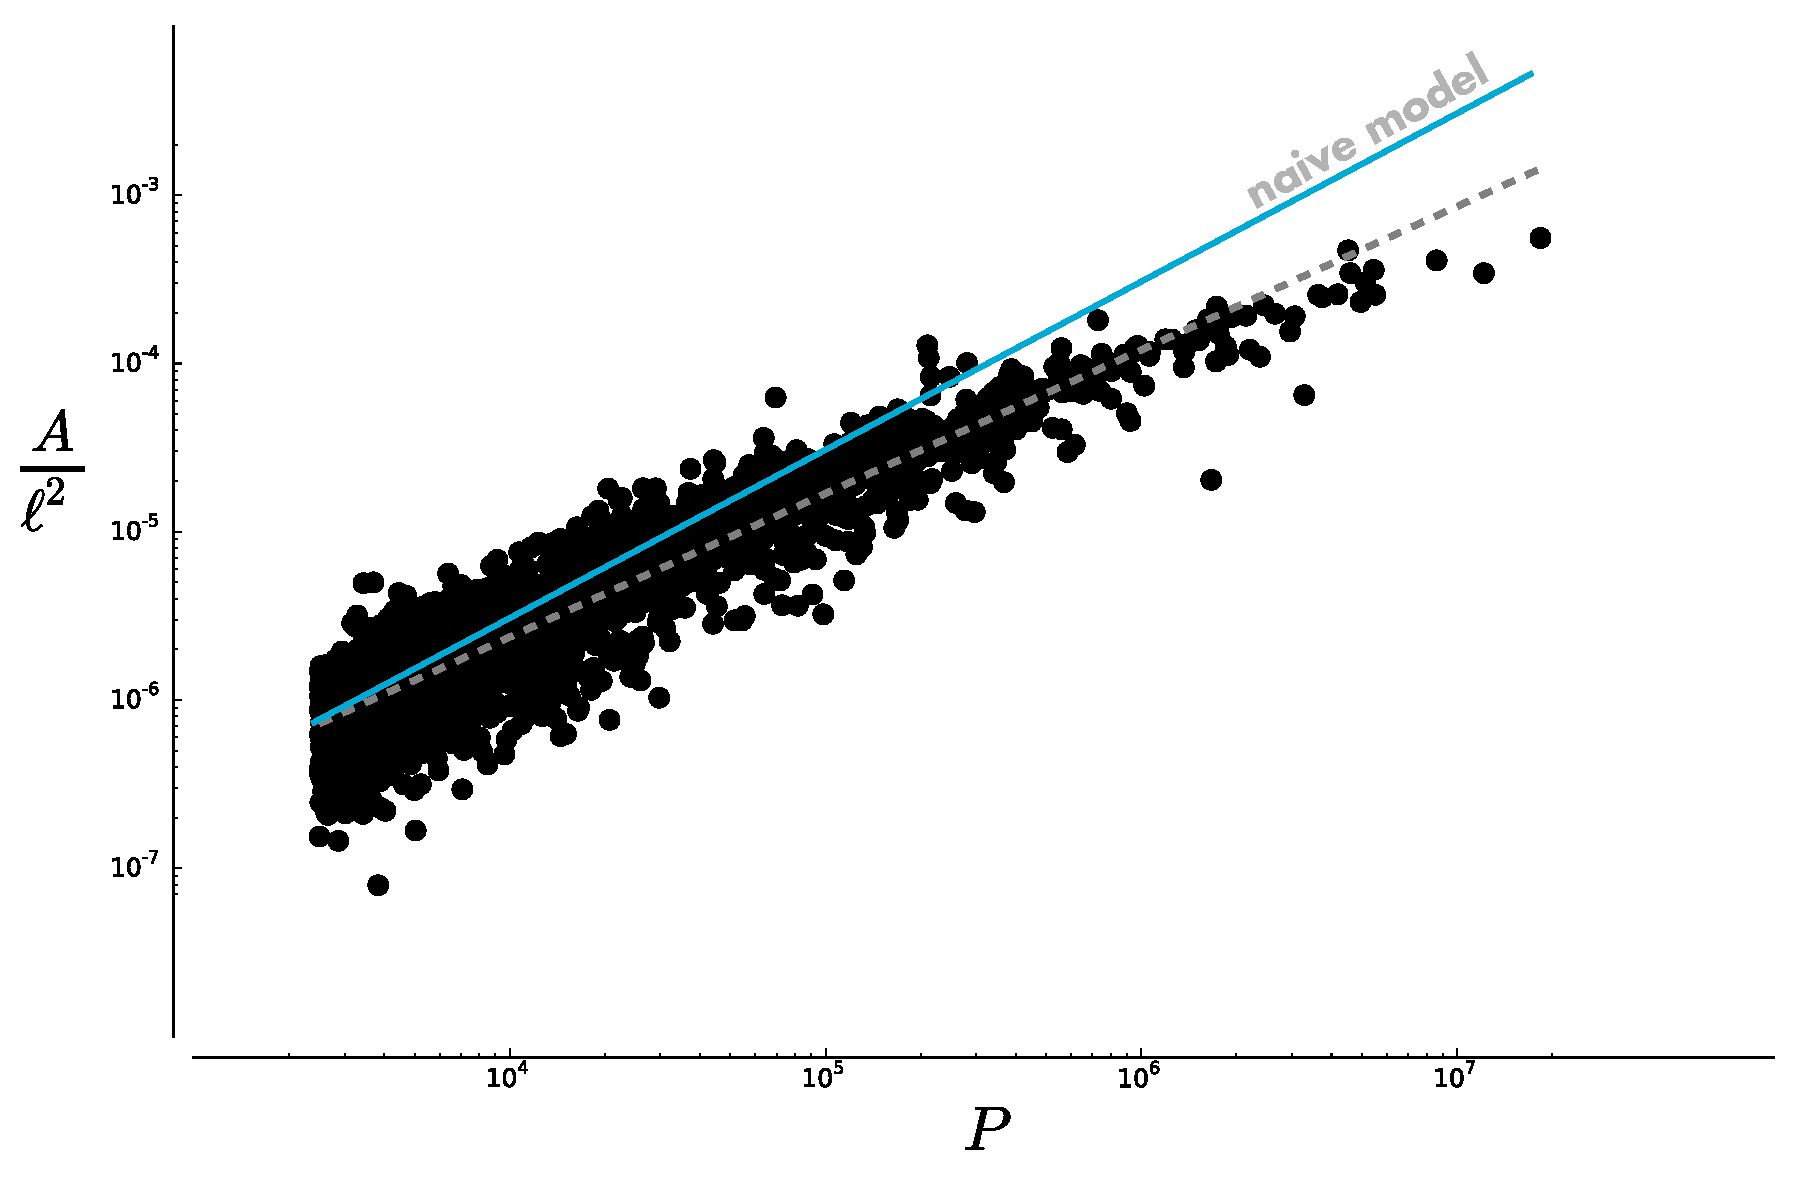
\includegraphics[width=\textwidth]{gfx/chapter-scaling/scaling_area.pdf}
    \caption{Scaling of the surface area of US urban areas with population size,
        and what would be expected with a naive model (blue solid line).
    A fit assuming a powerlaw dependence (dashed line) gives an exponent
    $\beta_A = 0.85 \pm 0.01\,(95\% CI)$.\label{fig:scaling_area}}
\end{figure}



\subsection{Total length of road}
\label{sub:total_length_of_road}

\paragraph{Naive model.} We would now like to estimate the total length $L_N$ of all the roads within a
city. If we consider that the network formed by streets is such that all the
nodes (intersections) are connected to their closest neighbour, the typical
length of a road segment is given by

\begin{equation}
    \ell_R \sim \sqrt{\frac{A}{N}}
\end{equation}

where $N$ is the number of intersections~\cite{Barthelemy:2008}. Previous studies of road networks in
different regions, and over extended time
periods~\cite{Strano:2012,Barthelemy:2013}, have shown that the number of
intersections is proportional to the population size. Therefore, the typical
length of a road segment (between two intersections) varies with the population
size $P$ as

\begin{equation} 
    \ell_R \sim \sqrt{\frac{A}{P}} 
    \label{eq:length_nodes}
\end{equation}

and the total length of the network $L_N \sim P\ell_R$ should then scale as

\begin{equation} 
    \frac{L_N}{\sqrt{A}} \sim \sqrt{P} 
\end{equation}

Using the naive scaling for the dependence of $A$ on population size given
previously in Eq.~\ref{eq:area_naive} we finally get 

\begin{equation} 
    L_N \sim P
\end{equation}

\paragraph{Reality.} Again, the naive argument does not compare well with
reality. We fit the data for US urban areas (see
Fig.~\ref{fig:scaling_lanemiles}) assuming a powerlaw dependence and find an
exponent

\begin{equation}
    \boxed{\beta_R \sim 0.765 \pm 0.033}
\end{equation}

Note that since the relation between the length and the number of nodes given by
Eq.~\ref{eq:length_nodes} and the relation between intersections and population
have been verified independently in the literature, the discrepancy likely is
due to the scaling of the surface area.

\begin{figure}
    \centering
    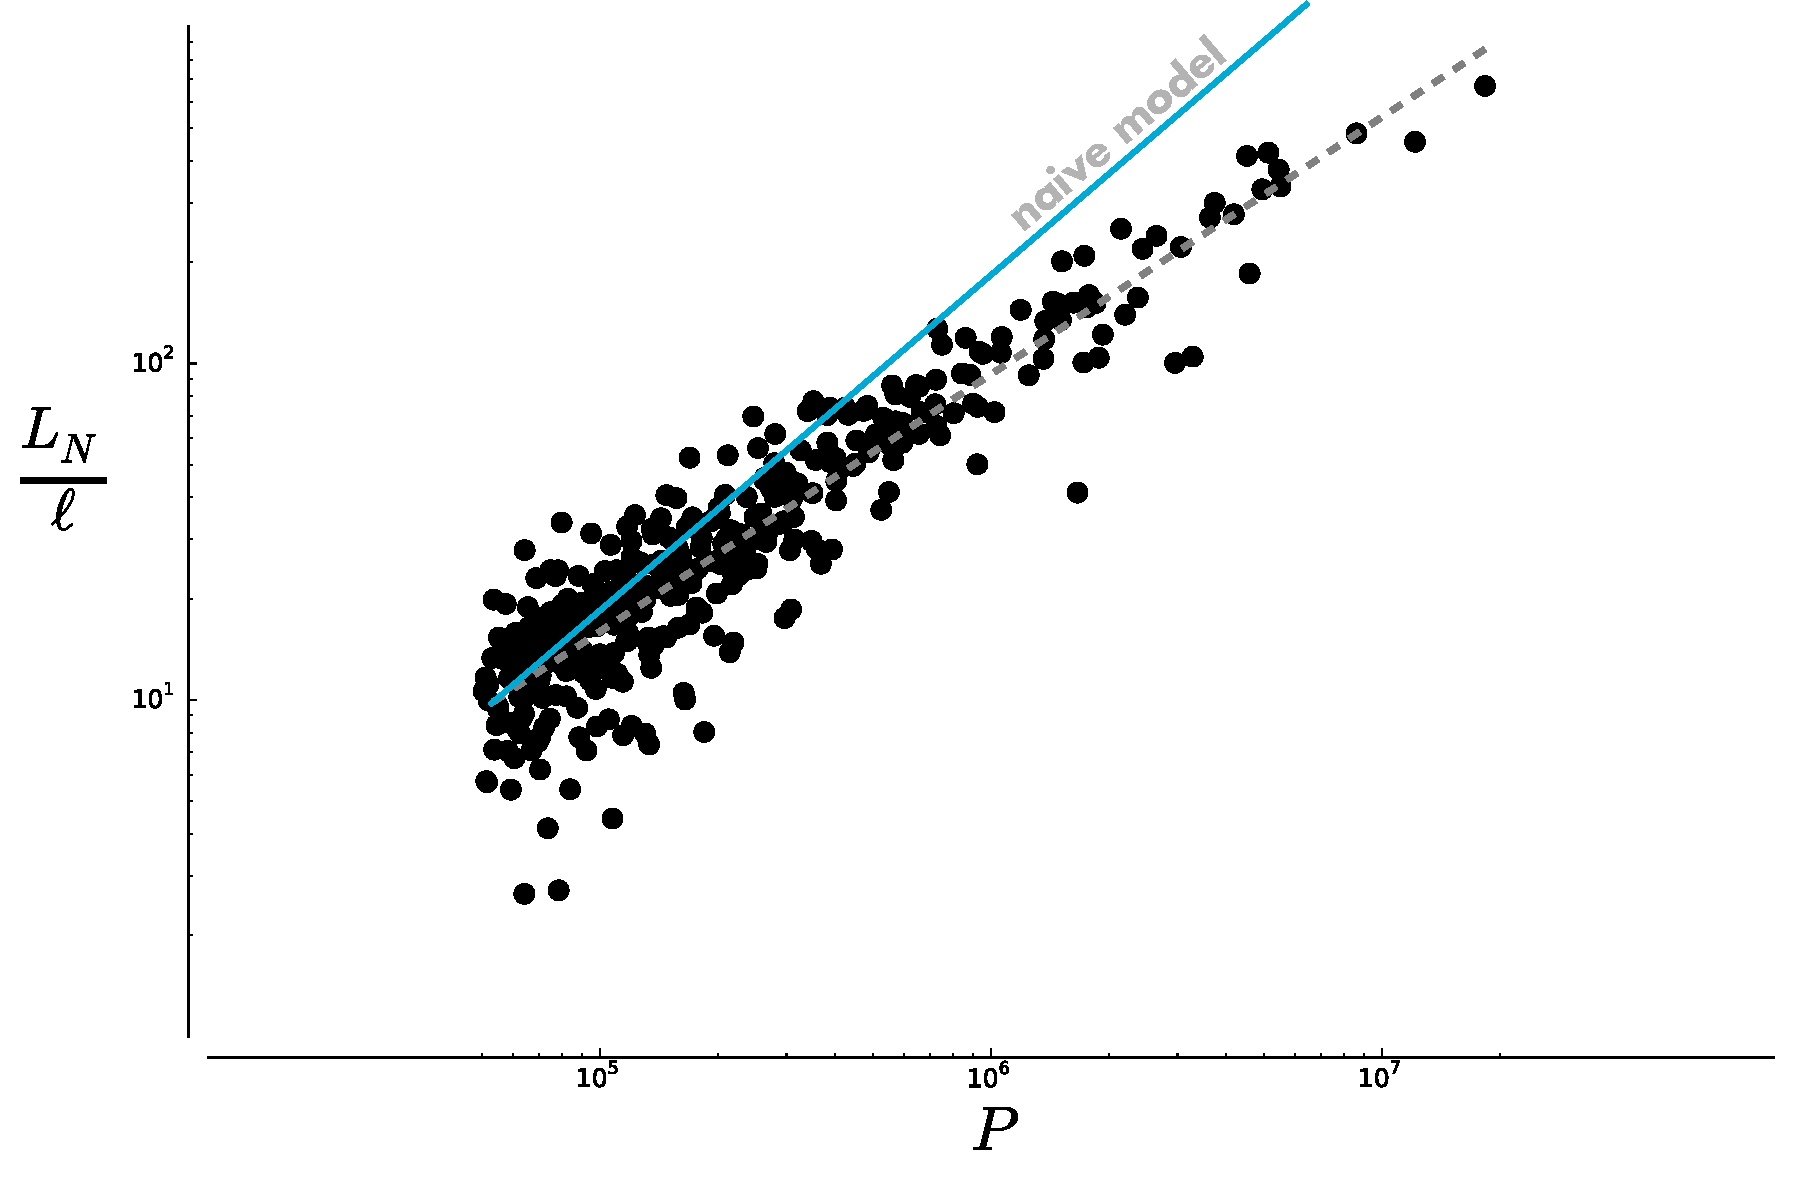
\includegraphics[width=\textwidth]{gfx/chapter-scaling/scaling_lanemiles.pdf}
    \caption{Scaling of the total length of roads in US urban areas versu the
    total population. A fit assuming a powerlaw dependence (dashed grey line)
gives an exponent $\beta_R \sim 0.765 \pm 0.033$ ($r^2=0.92$). The behaviour is
qualitatively different from what would be expected with a naive mode (solid
blue line).\label{fig:scaling_lanemiles}}
\end{figure}



\subsection{Total commuting distance}
\label{sec:total_length_driven}

The total commuting distance $L_{tot}$ is determined by two different
constraints. First the individual constraint: individuals have limitations and
their own behaviour, and are the ones who are making the decision about where
they are going to live and work.  However, the individuals' choices are limited
by the city structure itself, that is by how employment and residences are
spread across the city.



\subsubsection{Influence of the individual constraint} 

The first constraint on this distance comes from individuals's limitations and
behaviour. We make here the simple assumption that individuals choose their
residence and work place such that their total commuting distance is fixed (or
at least smaller than a certain value) and equal on average to $\ell_C$. In that
case, we would simply have

\begin{equation} 
    \frac{L_{tot}}{P} \sim \text{const.} = \ell_c 
    \label{eq:assum}
\end{equation}

(by constant, we mean independent from the population size of the city). As
surprising as it may seem, the data show that $L_{tot}/P$ can be considered
 independent from $P$ (with a value of approximately $23$ miles for
the US, see Fig.~\ref{fig:LtotoverP}), in agreement with the individual
constraint assumption (Eq. \ref{eq:assum}). This finding is also in agreement
with the results drawn from census data in Germany by~\cite{Wilkerson:2013}.
This does not mean, of course, that the distance driven is the same for every
city. As one can see on Fig.~\ref{fig:LtotoverP}, the fluctuations are quite
important between cities. But they do not depend on the population size.
Although this assumption of a constant distance is simple and verified on the US
data, we think that it deserves to be systematically tested on other datasets
for other countries and cities. 

\begin{figure}[!h]
    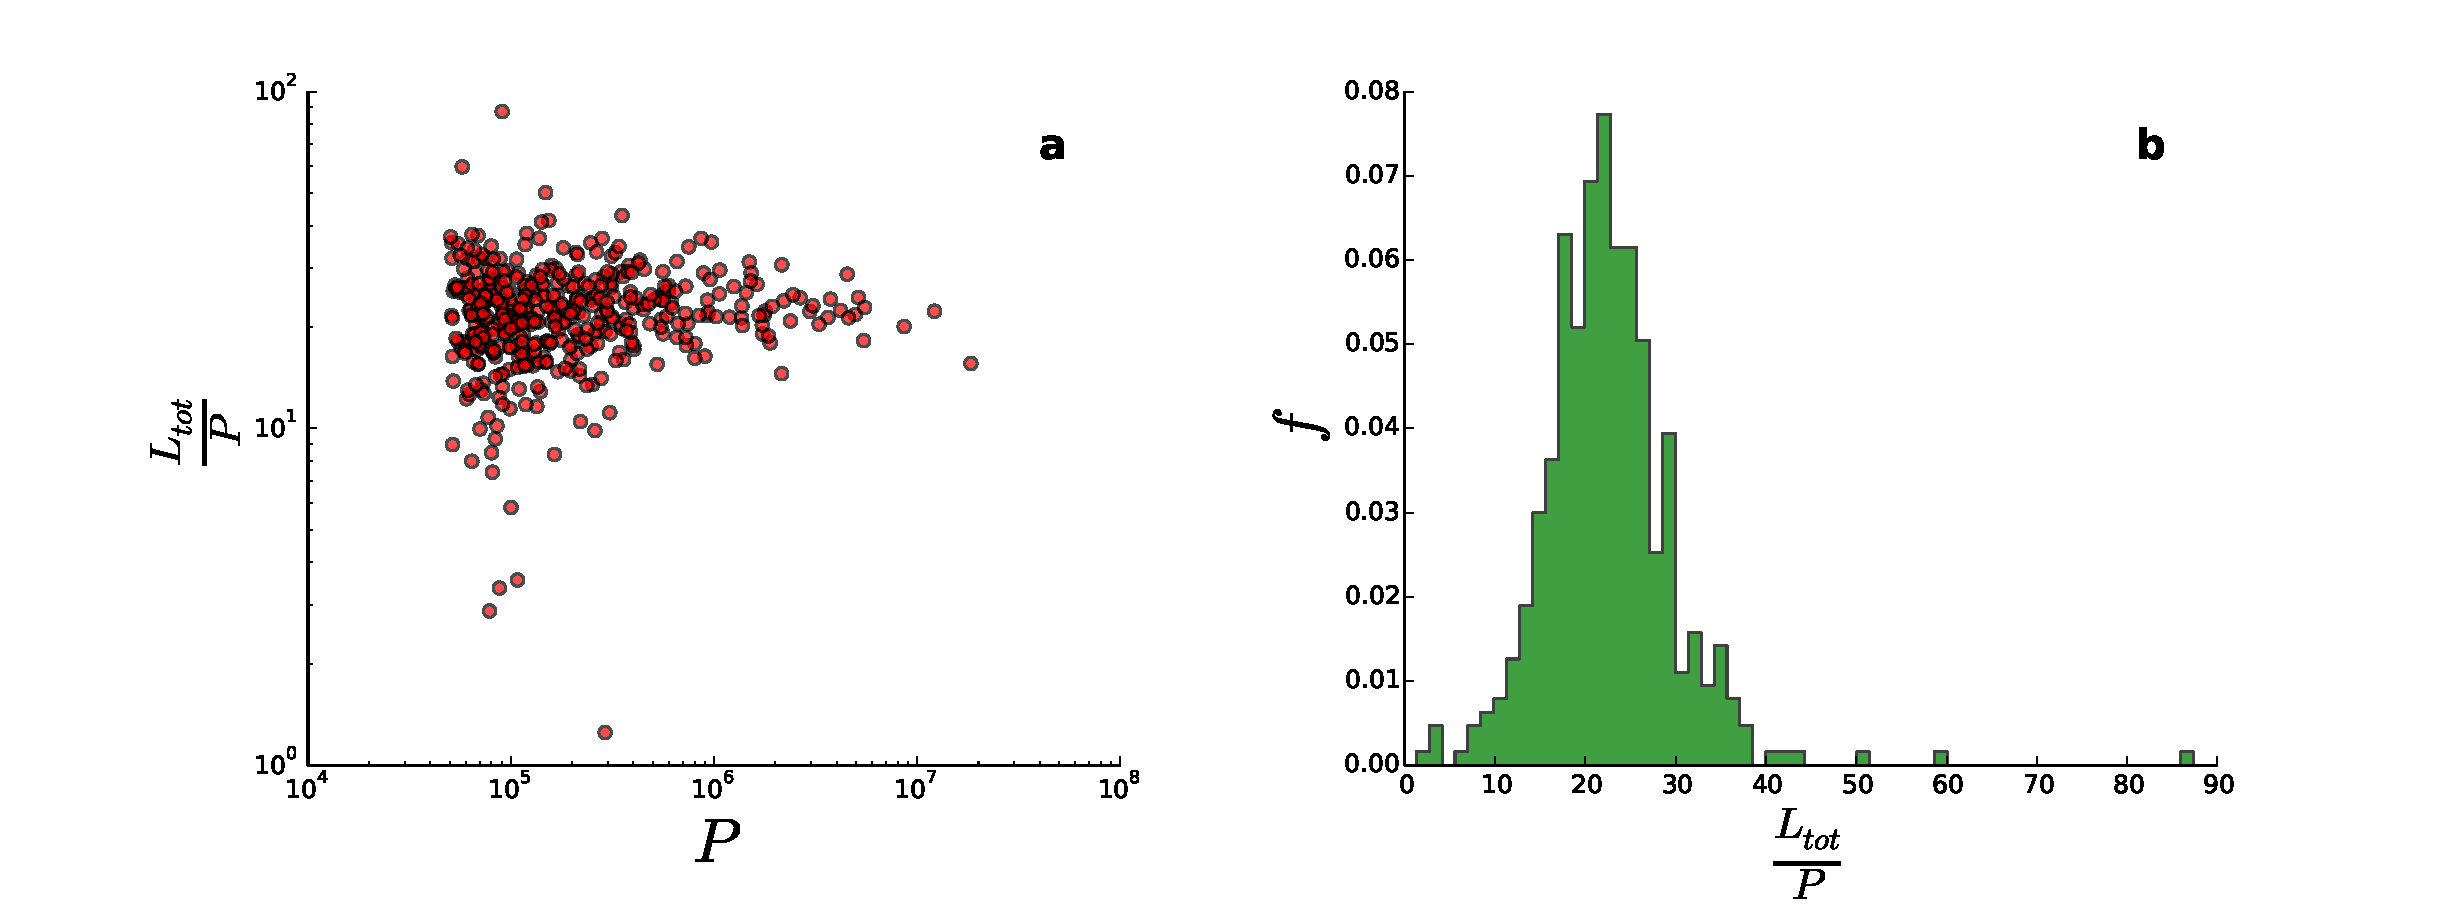
\includegraphics[width=1.0\textwidth]{gfx/chapter-scaling/figure_2.pdf}
    \caption{Constant daily driven distance per capita. (a) daily total driven
        distance per capita as a function of population for 441 urbanised area
        in the US in 2010. The data shown in the plot are compatible with a
    population-independent behaviour. (b) Histogram of the daily total driven
distance per capita for the same cities. The average daily driven distance for
these cities is $23$ miles, and the standard deviation $7$ miles.}
\label{fig:LtotoverP} 
\end{figure}



\subsubsection{Influence of the city structure}
\label{sub:influence_of_the_city_structure}

The easiest way to understand the influence of the city constraints is to
consider two limiting cases: on the one hand, the totally centralised
(monocentric) city where everyone goes to work to a single center, and the
totally decentralised city where everyone goes to work to the nearest
location (see Fig.~\ref{fig:monocentric_decentralised})~\cite{Samaniego:2008}.\\

\begin{figure}[!h]
    \centering
    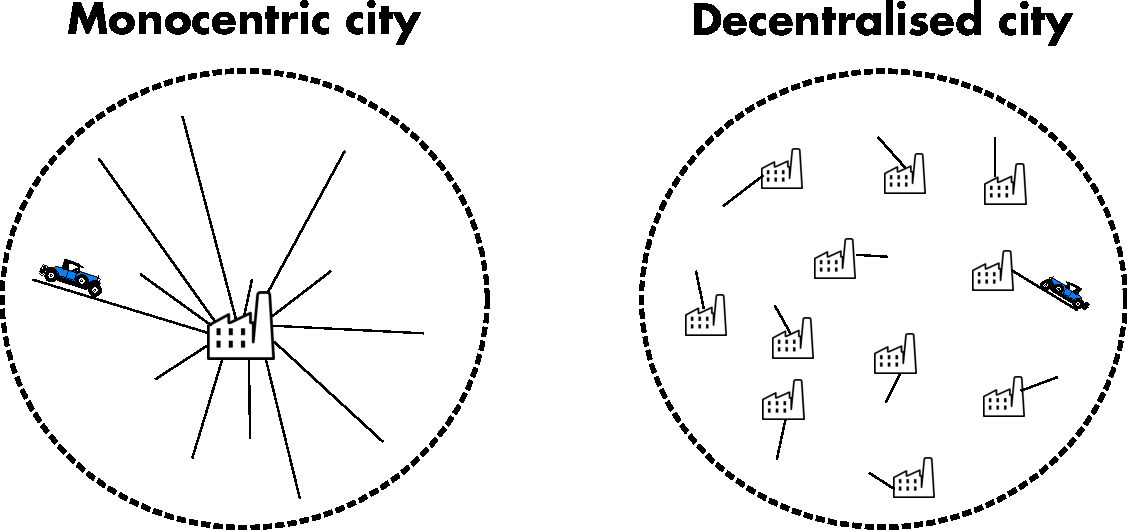
\includegraphics[width=1\textwidth]{gfx/chapter-scaling/monocentric-decentralised.pdf}
    \caption{Representation of the monocentric city (left) and the totally
    decentralised city (right), two extreme models for the shape of mobility
patterns.\label{fig:monocentric_decentralised}}
\end{figure}

\paragraph{Monocentric.} If we first assume that the city is monocentric, individuals are all commuting
to the same center and the typical commuting distance $\ell^m_c$ is controlled
by the typical size of the city of order $\sqrt{A}$, so that

\begin{equation} 
    \frac{L_{tot}^{m}}{\sqrt{A}} \sim P 
\end{equation}

\paragraph{Decentralised.} On the other hand, if we assume that the city is completely decentralised, the
typical commuting distance is of order the nearest neighbour distance
$\sqrt{A}/\sqrt{P}$, and we obtain

\begin{equation} 
    \frac{L_{tot}^{d}}{\sqrt{A}} \sim \sqrt{P} 
\end{equation}

\paragraph{Reality. } The scaling of the total driven distance for Urban Areas
(morphological definition) is shown on
Fig.~\ref{fig:scaling_Ltot_norm}, and the exponent sits between the ones of the
monocentric and decentralised cities

\begin{equation*}
    \boxed{\beta_L =  0.595 \pm 0.026\, (R^2 = 0.90)}
\end{equation*}


\begin{figure}
    \centering
    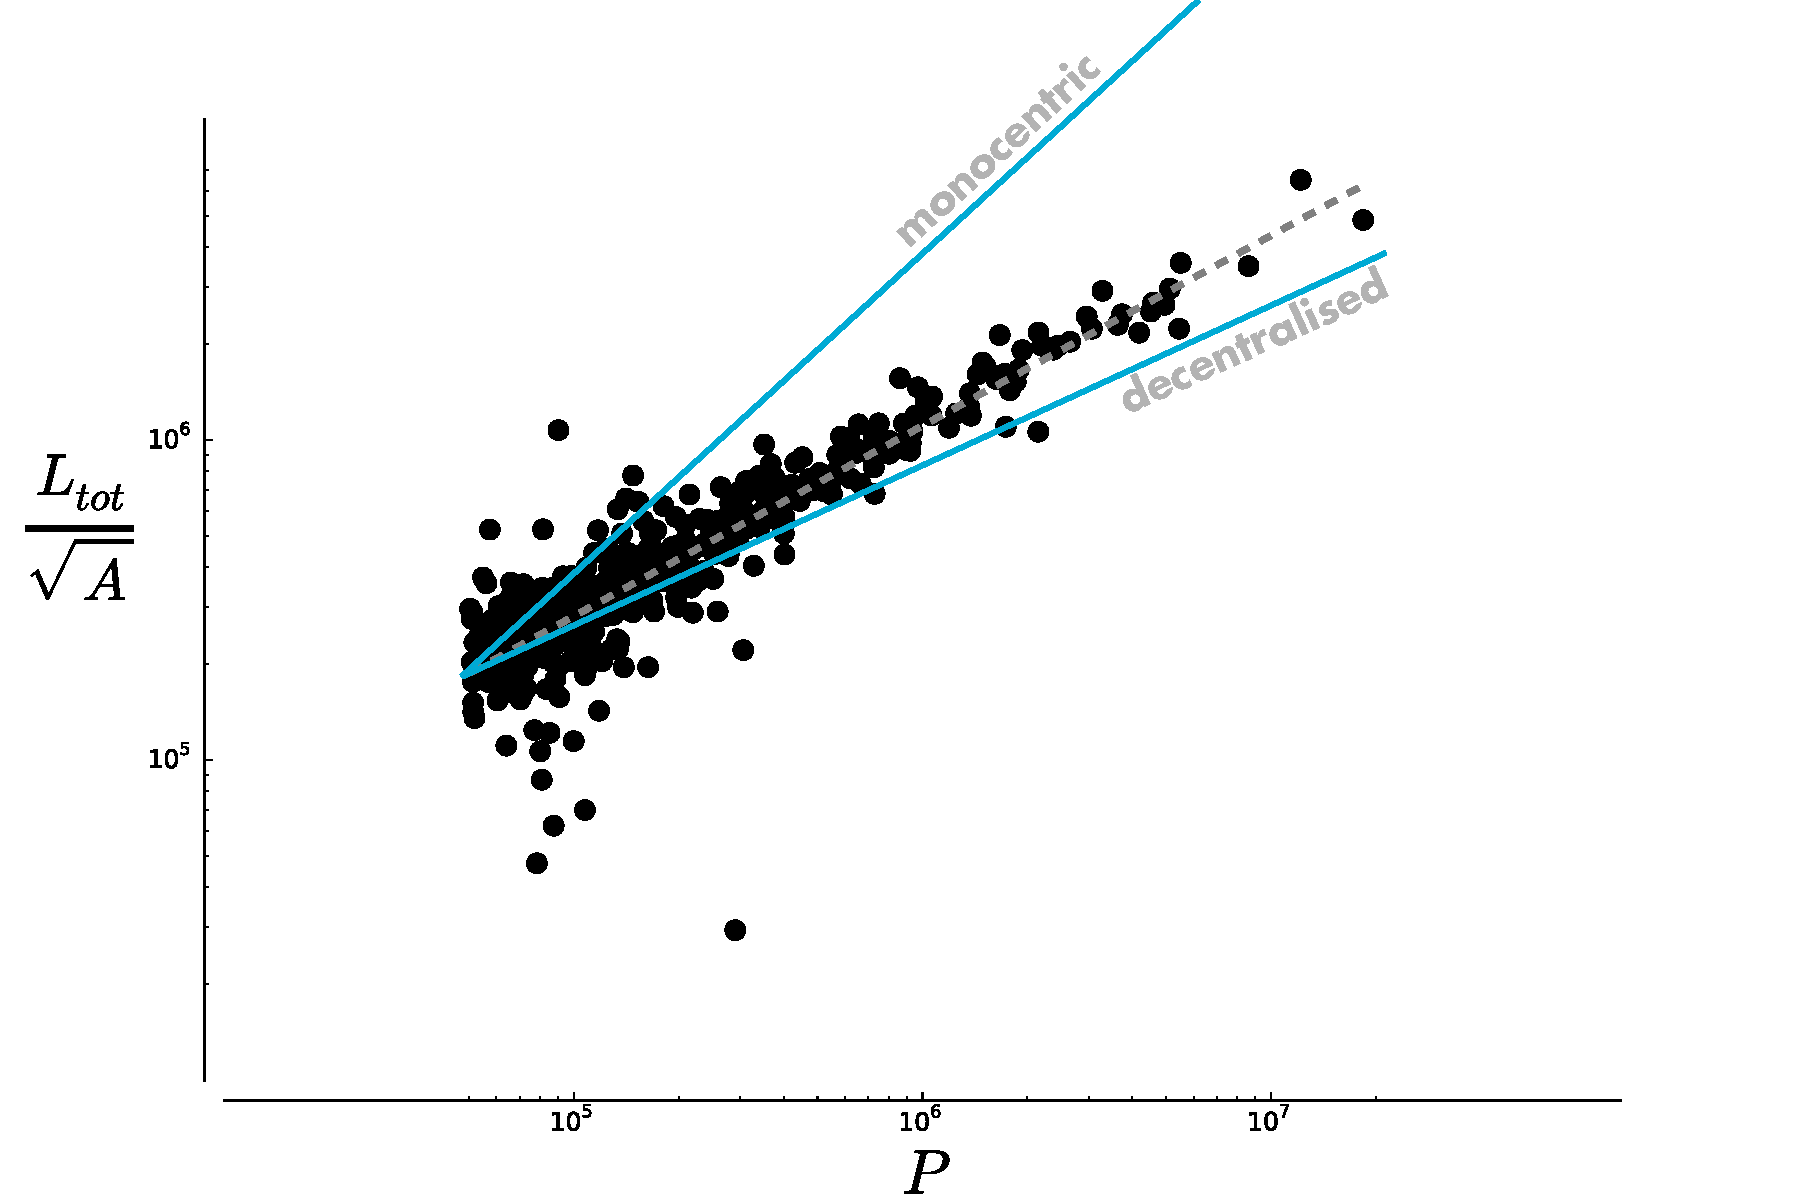
\includegraphics[width=0.9\textwidth]{gfx/chapter-scaling/scaling_commuting_norm.pdf}
    \caption{Scaling of the total yearly commuted distance normalised by the
    city's surface area with population size for US Urban Areas. The blue lines
show the behaviours that would be expected for a monocentric and a totally
decentralised city. The dashed line represents the fit assuming a powerlaw
dependence, which yields an exponent $\beta =  0.595 \pm 0.026\, (R^2 =
0.90)$.\label{fig:scaling_Ltot_norm}}
    
\end{figure}

This comes as another evidence -- different from that presented in
Chapter~\ref{chap:monocentric-introduction} -- that cities do not have a
strictly monocentric structure. In particular, this result cast some doubts
about the model by Bettencourt~\cite{Bettencourt:2013} which assumes implicitely that cities are always
monocentric. 

So far, so good. But how can we understand the non-trivial exponent that is observed? This is
where the limiting case are helpful: if the exponent sits between the ones that
would be obtained in a monocentric or decentralised city, surely, cities must
adopt an intermediate structure. Following the previous part on polycentricity,
there is an obvious candidate: the polycentric city (see
Fig.~\ref{fig:polycentric}).

\begin{figure}[!h]
    \centering
    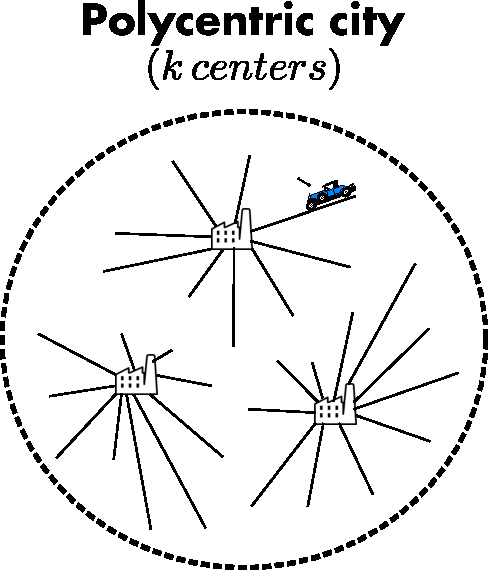
\includegraphics[width=0.4\textwidth]{gfx/chapter-scaling/polycentric.pdf}
    \caption{City with a polycentric structure, intermediate between the
    monocentric and totally decentralised situations. \label{fig:polycentric}}
\end{figure}

Let us consider a polycentric city with $k$ employment centers. The typical
distance commuted by individuals is given by

\begin{equation}
    \ell_c \sim \sqrt{\frac{A}{k}}
\end{equation}

So that

\begin{equation}
    \frac{L_{tot}}{\sqrt{A}} = \frac{P}{\sqrt{k}}
\end{equation}

Therefore if, as we showed in the previous part,  the number of centers
increases sublinearly with population, we would have a scaling of the form
$L_{tot}/\sqrt{A}\sim P^{\,\beta_L}$ where $\beta_L \in [1/2,1]$. One
can easily see that this expression is consistent with that of $A/\lambda^2$ and
$L_{tot}/P$ if

\begin{equation} 
    \beta_L = 1-\frac{\beta_A}{2} 
    \label{eq:consis} 
\end{equation}

which is indeed what we observe empirically (up to error bars). This preliminary
analysis thus leads us to the conclusion that, in order to compute the various
exponents, we need to better describe the structure of commuting patterns. In
other words, we need to find a description of cities that goes beyond the naive
monocentric or totally decentralized views, and which accounts for the observed
sub-linear scaling of the surface area $A$.






\section{Computing the exponents}

The previous results, in particular the behaviour of the total commuting length
with population, hint at the necessity to better describe the structure of the
mobility patterns to understand the previous scaling relationships. This is
exactly what the model presented in the previous does.
Using the relation that we derived for the number of centers, we will see how we
can understand the values of the exponents presented earlier in this chapter. We
will also see how the model allows us to understand the scaling of other
quantities, namely the total time spent in traffic and the total $CO_2$
emissions due to transportation.

\subsection{Area}

At this stage, the number of centers is a function of population and the area

\begin{equation}
    k = F\left(A,P\right)
\end{equation}

and we need an additional equation in order to get a closed system. Here we
focus on the area and its evolution with the population size, which reflects the
growth process of the city. In the following, we will investigate two different
approaches. It is worth noting that both approaches give results in qualitative
agreement, showing that some stylized facts ---such as super- or sublinearity---
are very robust.\\ 

\paragraph{Fitting procedure.}

In the absence of knowledge of the processes responsible for urban sprawl, we
can assume that the area behaves as 

\begin{equation}
    A \sim P^{\,a}
    \label{eq:fit}
\end{equation}

where $a$ is the exponent to be determined, through fits on data. The empirical
value for the exponent for the US data is $a\simeq 0.85$. Once this exponent is
given we can then compute the various exponent for the quantities of interest
(see the following and table 2). We get for the number of centers $k$

\begin{equation}
    k \sim P^{\frac{\mu + a/2}{\mu+1}}
\end{equation}

which is sublinear as long as $a<2$, in agreement with the empirical results for
US cities. As we will see, this approach yields the same qualitative behaviours
as those predicted with the method of the next section. In other words, even if
the main mechanism behind urban sprawl is not congestion, the conclusions of
this paper are not affected as long as the area scales \emph{sublinearly} with
population.\\


\paragraph{Coherent growth.}

Let us now assume that the scaling of $A$ with population is determined by the
number of activity centers and the constant commuting length of individuals.
This means that the growth of the area is controlled by the appearance of new
activity centers. if we assume that a city is organized around $k$ activity
centers and that the attraction basin of each of these centers are spatially
separated~\cite{Louf:2013_polycentric}, we then have  $A \sim k\, A_1$ where $A_1$ is the
area of each subcenter's attraction basin. This area $A_1$ is related to the
average individual commuting distance by $\sqrt{A_1} \sim L_{tot} / P$, and we
obtain

\begin{equation}
    A \sim k\,  \left( \frac{L_{tot}}{P} \right)^2 = k\, \ell_c^2
    \label{eq:area_poly}
\end{equation}

This leads to expression for the number of centers

\begin{equation}
    k \sim P^{\frac{2 \mu}{2\mu+1}}
\end{equation}

which is always smaller than $1$, also in agreement with the empirical results
for US cities. We can now also compute the scaling of the surface area

\begin{equation}
    \frac{A}{\ell_c^2} \sim \left( \frac{P}{c} \right)^{\frac{2 \mu}{2\mu+1}}
\end{equation}

We further assume that $L_{tot} / P$ is a fraction of the longest possible
journey $\ell$ individuals can afford, that is to say 

\begin{equation}
    \ell_c \sim \ell
\end{equation}

It is important to note that if $\ell_c$ is independent from $\ell$, the
quantitative predictions of our model would still hold. 

The final expression for the area is then here given by

\begin{equation}
    \frac{A}{\ell^2} \sim \left( \frac{P}{c} \right)^{\,2\,\delta}
    \label{eq:area}
\end{equation}

where $\delta=\frac{\mu}{2\mu+1}$. The exponent $\delta$ is smaller than $1/2$
whatever $\mu\geq 0$, which implies that the density of cities increases
\emph{sublinearly} with population. In other words, the density of cities
\emph{increases}  with population. We verify this prediction in Table 2, with
data about land area of urbanized areas in the US (Figure 2). We find $2
\delta_{emp} = 0.85 \pm 0.01\; (95\%\, CI)$ which is not too far from the
theoretical value $2\delta_{th} = 0.64 \pm 0.12\; (95\%\, CI)$, equal to
$\alpha$ in this case.\\

Because the area of an urban system results from centuries of evolution, we do
not a priori expect our model --where individual vehicles are assumed to be the
only vector of mobility-- to give a prediction valid for all countries and all
times. Nevertheless, these results give us reasons to believe that the spatial
structure of the journey-to-work commuting should still be the dominant factor
in the dependence of land area on population. In the following, we will use the
above numerical value to compute other scaling exponents.


\subsection{Total commuting distance}

Using Eq.~\ref{eq:assum} and Eq.~\ref{eq:area} we are now able to compute $L_{tot}/\sqrt{A}$

\begin{equation}
    \frac{L_{tot}}{\sqrt{A}} = P\; \left(\frac{P}{c}\right)^{-\delta}
    \label{eq:travelled_length}
\end{equation}

We plot $L_{tot} / \sqrt{A}$ for urbanized areas in the US on Figure 2, and one
can check in Table 2 that the exponent predicted from the previously measured
value of $\alpha$ agrees well with the exponent measured on the data.


\subsection{Total length of roads}

If we use the previously derived expression for the area $A$, we find

\begin{equation}
    L_N \sim \ell \; \sqrt{P}\; \left(\frac{P}{c}\right)^{\,\delta}
\end{equation}

The quantity $\delta$ is less than $1/2$, which implies that $L_N$ scales
\emph{sublinearly} with the city's population size. In other words, larger
cities need less roads per capita than smaller ones: we recover the fact that
agglomeration of people in urban centers involves economies of scale for
infrastructures. Within the fitting assumption (Eq.\ref{eq:fit}), we would
obtain $(1+a)/2$.

\subsection{Total delay due to congestion}

\begin{figure}
    \centering
    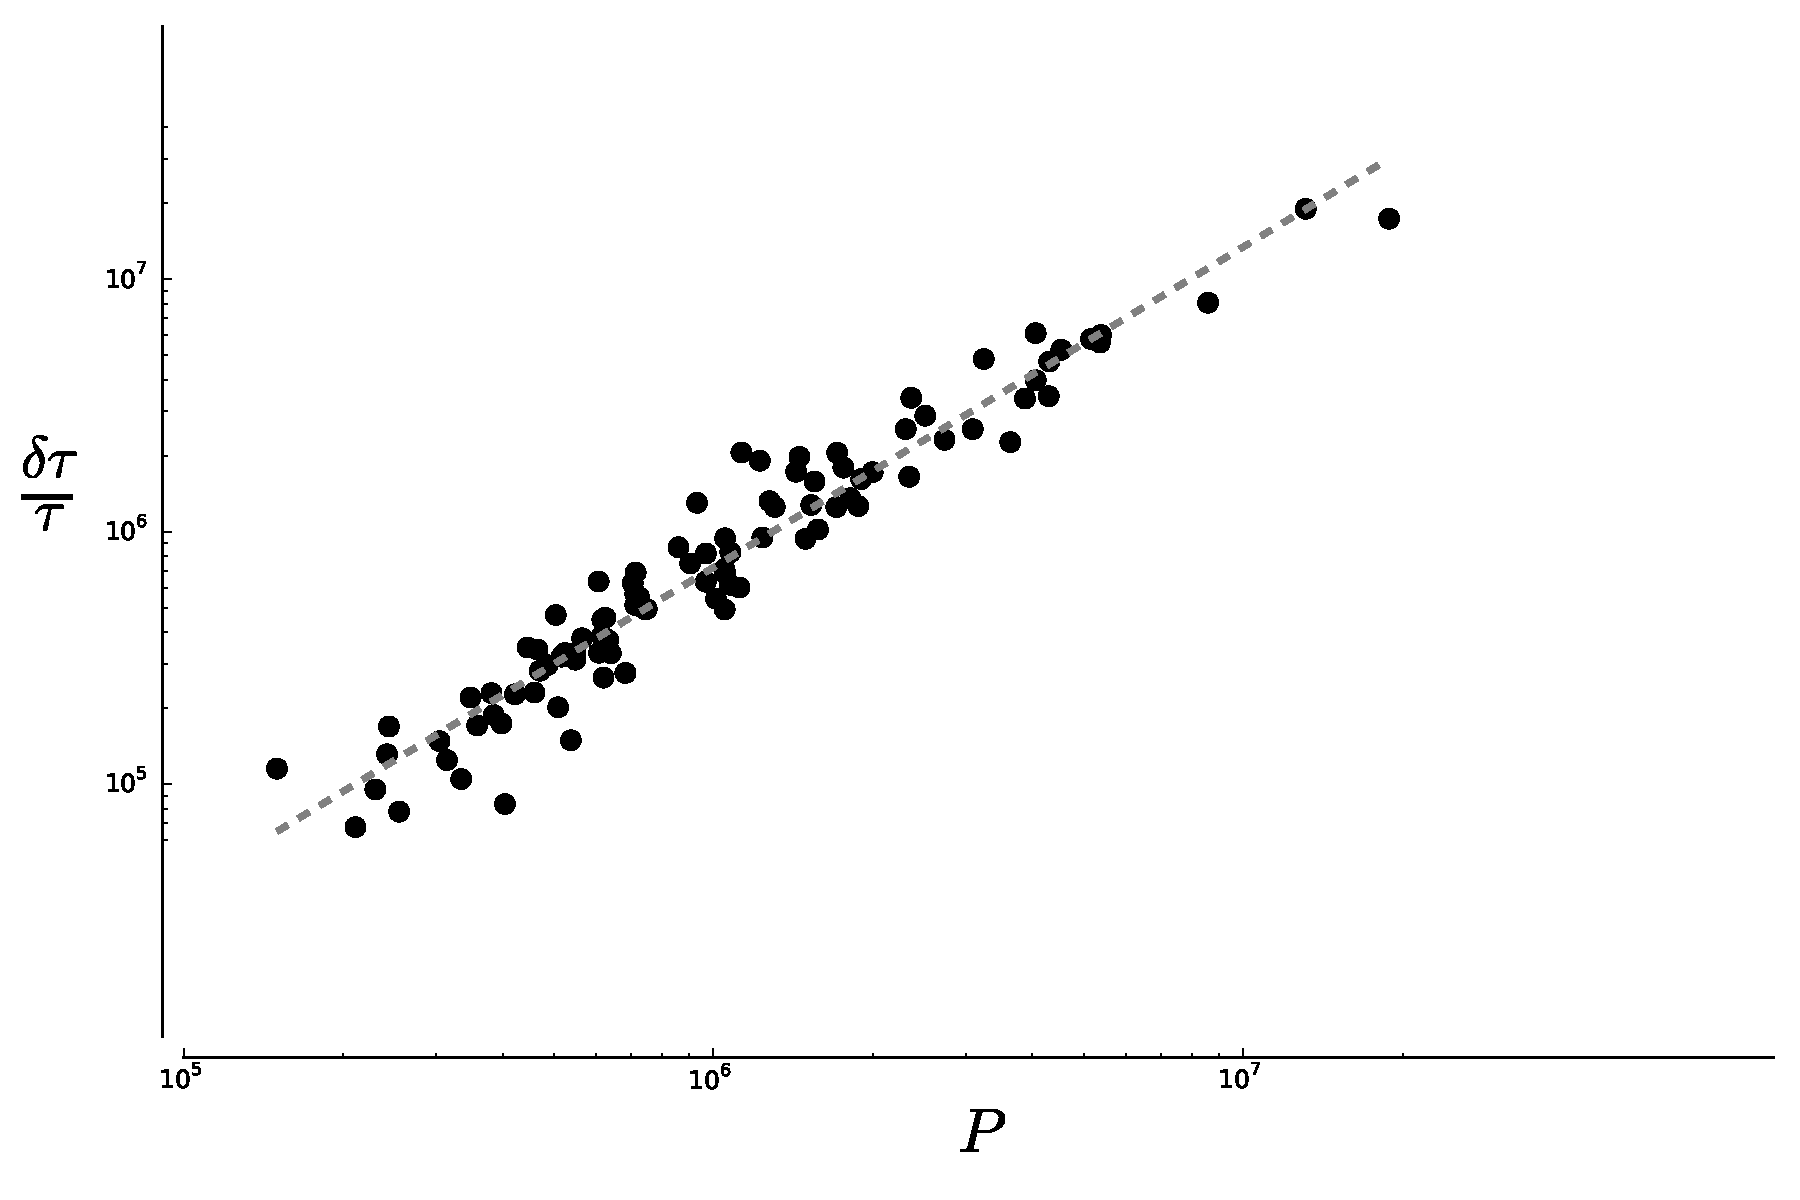
\includegraphics[width=\textwidth]{gfx/chapter-scaling/scaling_delay.pdf}
    \caption{Scaling of the total delay due to congestion of US urban areas with
    population size. \label{fig:scaling_delay}}
\end{figure}

Unfortunately, agglomeration in cities does not only generate economies.
Congestion, for instance, is a major diseconomy associated with the
concentration of people in a given area. A simple way to quantify the
impairement caused by traffic congestion is through the total delay it
generates. If we make the first order approximation that the average free-flow
speed $v$ is the same for everyone, the total delay due to congestion is given
--according to our model-- by

\begin{equation} 
    \delta \tau = \frac{1}{v} \sum_{i,j} d_{ij} \left(\frac{T_j}{c} \right)^\mu 
\end{equation}

If we assume that all the centers share the same number of commuters --a
reasonable assumption within our model~\cite{Louf:2013}-- we obtain

\begin{equation} 
    \delta \tau \sim \frac{L_{tot}}{v} \left( \frac{P}{k}
\right)^{\mu} 
\end{equation} 

which, using the expressions for $L_{tot}$ and $A$
given in Eq.~\ref{eq:travelled_length} and Eq.~\ref{eq:area} respectively, gives

\begin{equation} 
    \delta \tau \sim \frac{\ell\; P}{v}\;\left(\frac{P}{c}\right)^{\delta} 
\end{equation}

The total commuting time corresponding to the same distance but without
congestion scales as $\tau_0\sim L_{tot}$ and thus less rapidly than the total
delay which scales \emph{super-linearly} with population (even when
polycentricity is taken into account). This means that, for the largest cities,
delays due to congestion actually dominate the time spent in traffic, and that
economical losses \emph{per capita} due to the time lost in congestion --and the
corresponding strain on people's life-- increase with the size of the city. 

In the fitting assumption Eq. \ref{eq:fit}, and using the same arguments for the
calculation of $\delta\tau$, we easily obtain for the exponent the value
$1+\frac{\mu}{\mu+1}\left(1-\frac{a}{2}\right)$.

\subsection{Transport related $CO_2$ emission. Gasoline consumption}

Another diseconomy associated with congestion is the quantity of $CO_2$ emitted by cars and the gasoline consumed by motor vehicles. This amount not only depends on the distance that has been driven, but also on the traffic during the journey. It indeed turns out that for the same length driven, a car burns more oil when the traffic is heavy than when the road is clear.  Within our model, the presence of traffic is seen in the time spent to cover a given distance, and we write that the quantity of $CO_2$ emitted by a vehicle is proportional to the total time spent in traffic, leading to

\begin{equation}
    Q_{CO_2}  = q \sum_{i,j} d_{ij} \left[ 1+ \left( \frac{T_j}{c} \right)^\mu \right]
\end{equation}

where $q$ is the average quantity of $CO_2$ produced per unit time. In the
polycentric case with $k=k(P)$ subcenters, the typical trip length
$\overline{d_{ij}}$ is given by $\sqrt{A/k}$ and we obtain

\begin{equation}
    Q_{CO_2} = q\, \ell\, P \left[ 1 + \left(\frac{P}{c}\right)^{\delta} \right]
\end{equation}

The first term in brackets is a constant, and the quantity of $CO_2$ is thus
dominated by congestion effects at large populations

\begin{equation}
    Q_{CO_2} \sim q\; \ell\; P \left(\frac{P}{c}\right)^{\delta}
\end{equation}

and the total daily transport-related $CO_2$ emission per capita thus scales as 

\begin{equation}
    \frac{Q_{CO_2}}{P} \propto  q\ell \left(\frac{P}{c}\right)^{\delta}
\end{equation}

The quantity of $CO_2$ emitted per capita in cities thus increases with the size
of the city, a consequence of congestion. This prediction agrees with the
exponent we measure (Figure 3) on data gathered for US and OECD cities (Data
about the area and population of urbanised areas can be found  on the Census
Bureau website \cite{DataUSA1}, data about congestions in urban areas can be
found in the Urban Mobility Report \cite{DataUSA2}, and data about the total
lane miles and the daily total miles driven in urbanized areas can be found on
on the Federal Highway administration website \cite{DataUSA3}). We are aware
that the scaling of $CO_2$ with population size is controversial, with results
varying from one study to another. Although a systematic meta-analysis of these
results is beyond the scope of this paper, we note that the authors
of~\cite{Fragkias:2013} are concerned with the total emissions of $CO_2$, while
this paper is only concerned with emissions due to transportations. Moreover,
our prediction agrees well with the exponent of $1.33$ measured by the authors
of~\cite{Oliveira:2014} on the same dataset, but with a different definition of
cities. Finally, our prediction also agrees with measurements made in
\cite{Rybski} for developing countries. 

\begin{figure}
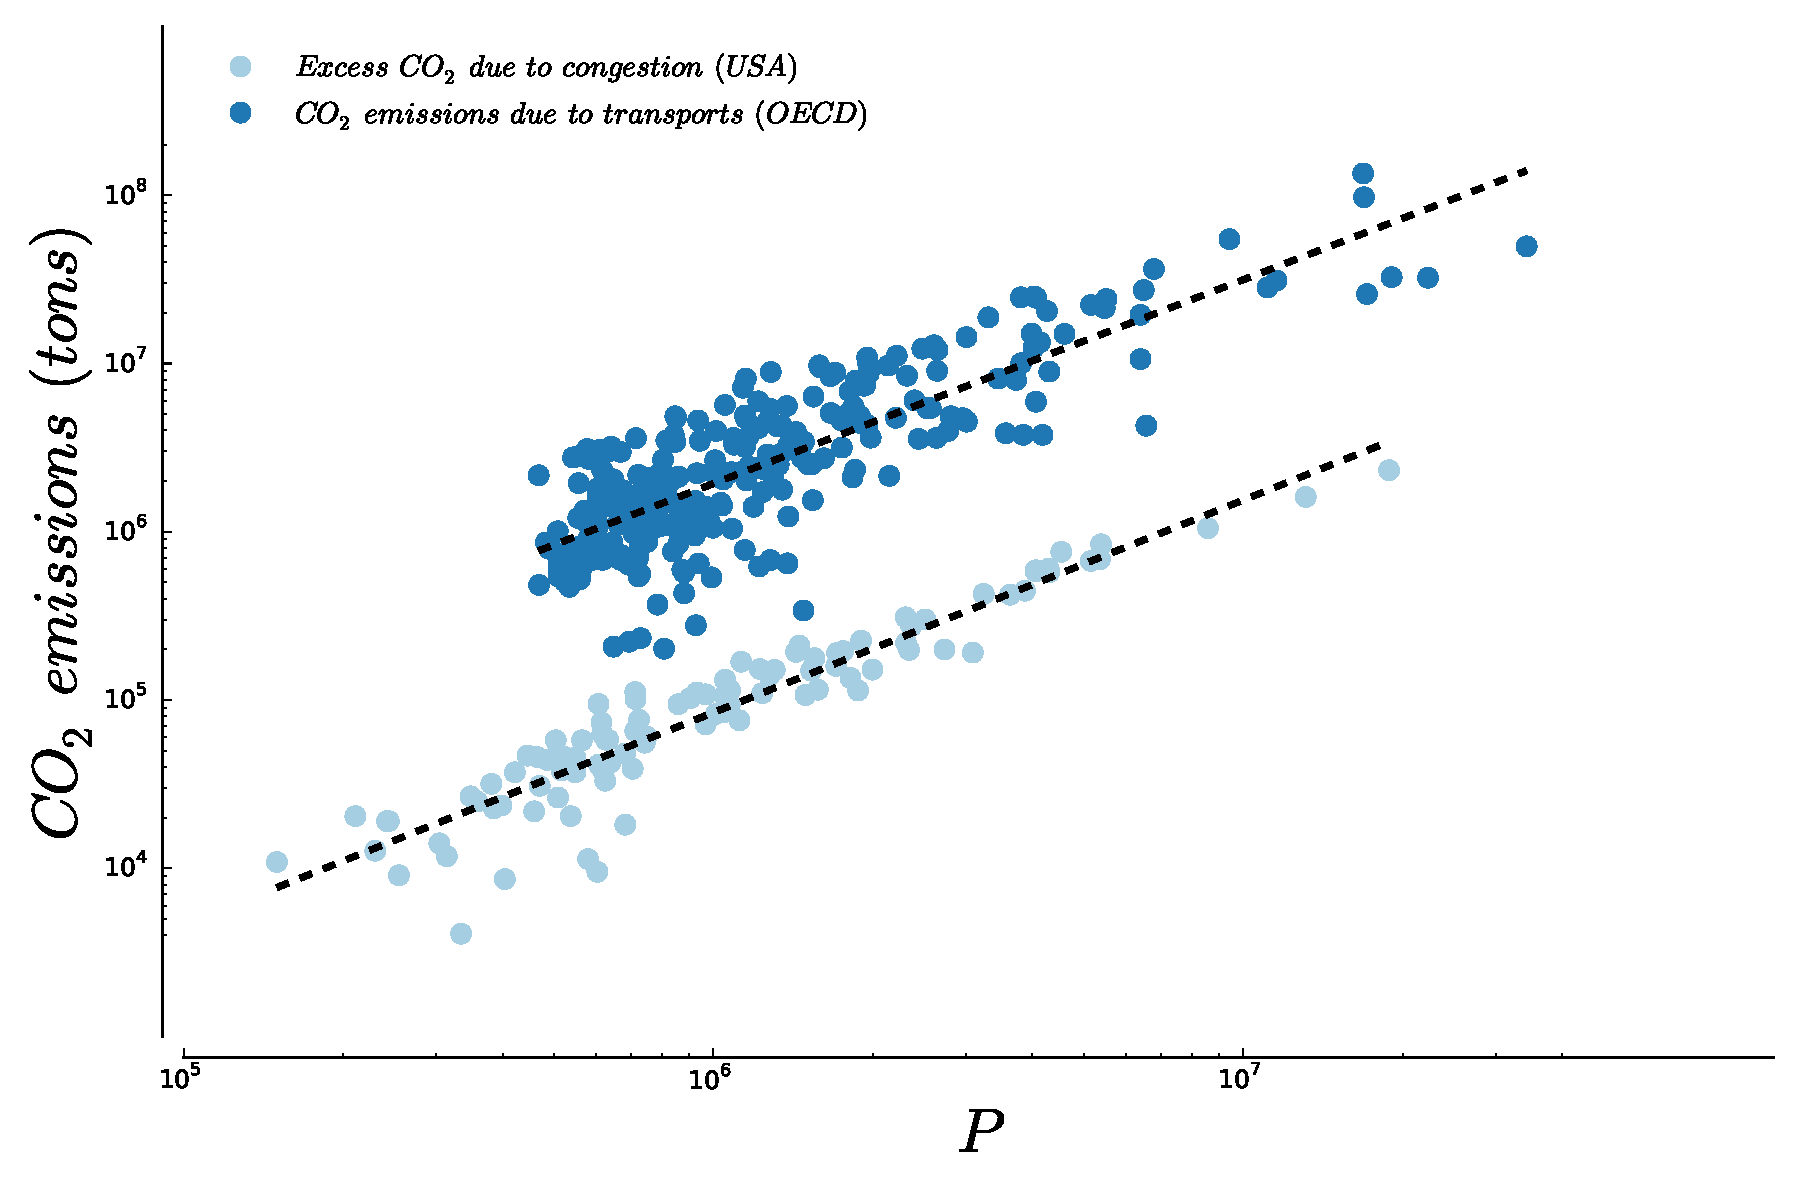
\includegraphics[width=0.9\linewidth]{gfx/chapter-scaling/scaling_co2.pdf}
\caption{Variation of $CO_2$ emissions due to transport with city size. In blue, excess $CO_2$ (in tons) due to congestion, as given by the Urban Mobility Report (2010) for 101 metropolitan areas in the US~\cite{DataUSA2}. In green, we show the estimated $CO_2$ emissions (in tons) due to transports, as given by the OECD for 268 metropolitan areas in 28 different countries (Data about the total $CO_2$ emissions due to transportation in major metropolitan area in the OECD can be found online~\cite{OECD}). The dashed yellow lines represent the least-square fit assuming a power-law dependency with multiplicative noise, which gives respectively $Q_{CO_2} \sim P^{1.262 \pm 0.089} (r^2=0.94)$ for the US data and $Q_{CO_2} \sim P^{1.212 \pm 0.098} (r^2=0.83)$ for the OECD data.}
\end{figure}



\section{Discussion}

\subsection{Travel-time budget and congestion}

\subsection{Newman \& Kenworthy}

\begin{figure}
    \centering
    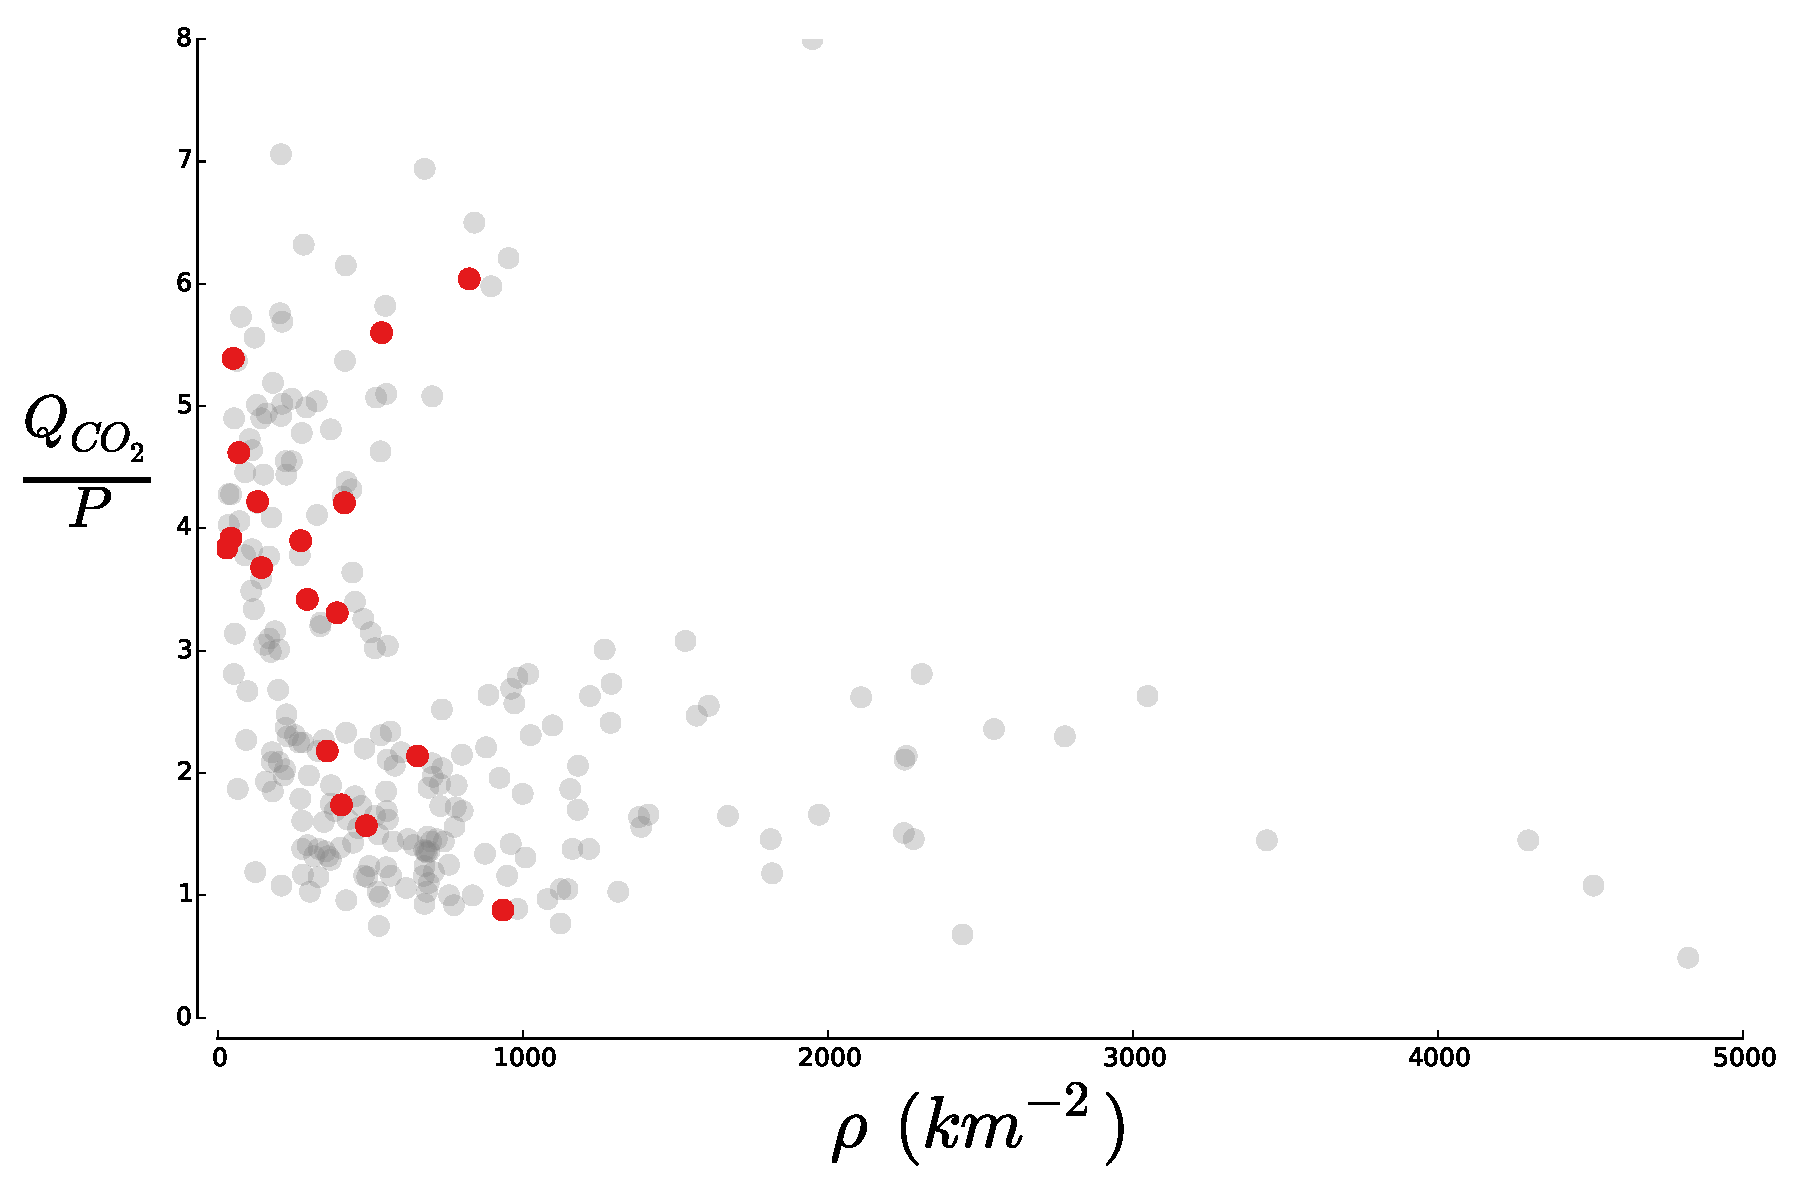
\includegraphics[width=\textwidth]{gfx/chapter-scaling/newman_kenworthy.pdf}
    \caption{Per capita $CO_2$ emissions versus the population density of cities
    belonging to OECD countries. The cities also present in the Newman \&
    Kenworthy dataset are represented in red. This curve casts serious doubt on
the fact that energy consumption are a simple funtion of
density.\label{fig:newman_kenworthy}}
\end{figure}

Another important related quantity is the the consumption of gasoline which in
principle is proportional to the emission of $CO_2$ and the time spent driving.
The total daily gasoline consumption is then given by

\begin{equation} 
    Q_{gas} \sim q\; \ell\; P \left(\frac{P}{c}\right)^{\delta}
\end{equation}

where $q$ is the average quantity of gasoline needed per unit time. From this
expression, we see that the total daily gasoline consumption per capita scales
as

\begin{equation} 
    \frac{Q_{gas}}{P}\sim \ell\, \sqrt{\frac{P}{\rho}} = \ell
\sqrt{A} 
    \label{eq:nk_area}
\end{equation}

and is therefore not a simple function of the city density, in contrast with
what was suggested by the seminal paper of Newman and
Kenworthy~\cite{Newman:1989}. At this stage however, more data about gasoline
consumption is needed to test this prediction and draw definitive conclusions.

\begin{figure}
    \centering
    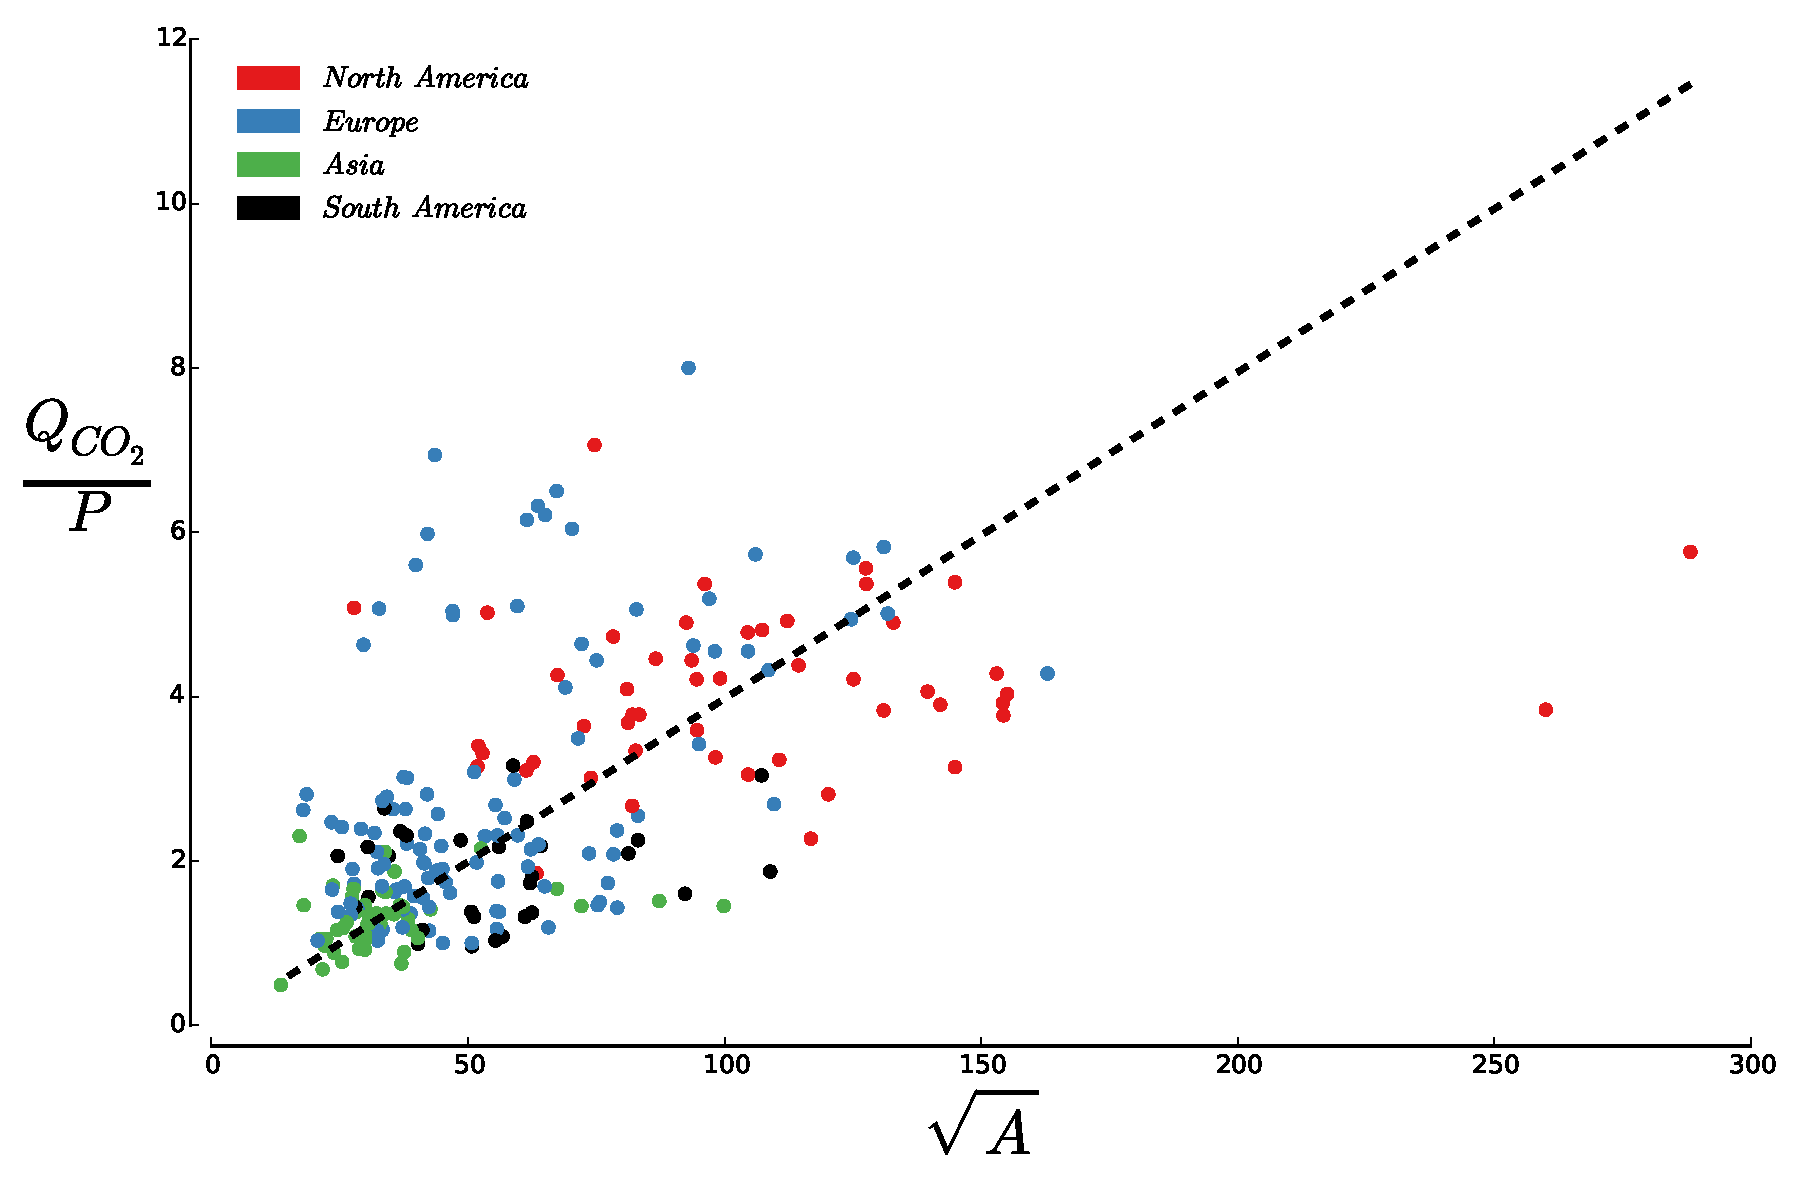
\includegraphics[width=\textwidth]{gfx/chapter-scaling/nk_model.pdf}
    \caption{Per capita $CO_2$ emissions versus $\sqrt{A}$ for cities of
    countries that belong to the OECD. The dashed line represents the obtained
linear fit, as predicted by Eq.~\ref{eq:nk_area} ($r^2=0.55$). The agreement is
poor, which may be due to the fact that cities all belong to different systems
of cities (and thus have a different prefactor).\label{fig:nk_model}}
\end{figure}

\subsection{Monocentric versus polycentric}

Although polycentricity emerges naturally from our model as a result of congestion, many circumstances can prevent or foster the appearance of new activity centers in a city. There are many debates as to whether policies should favour polycentric or monocentric developpement of cities. Most of them are based on ideologies and opinions about how cities should be, very few are based on a quantitative understanding of the city as a complex system. Although this only represents a small part of the debate, our model allows to quantify the effect of polycentricity on the total delay due to congestion.

We can indeed compute the total delay due to congestion in the case of a monocentric configuration. In this situation, all the population commutes to a single destination $1$ and we have

\begin{equation}
    \delta \tau_{mono} = \frac{1}{v}\; \sum_i d_{i1} \left(\frac{P}{c} \right)^\mu = L_{tot} \left(\frac{P}{c} \right)^\mu
\end{equation}

It follows, using the expression given above for $L_{tot}$

\begin{equation}
    \delta\tau_{mono} = \frac{\ell}{v}\; P^{1+\mu}
\end{equation}

From the fact that $1+\mu > 1+\frac{\mu}{2\mu+1}$, we indeed find that the total delay due to
congestion is worse for monocentric cities than it is for polycentric cities with the same population, which agrees with the usual intuition. More precisely the ratio of delays is given by

\begin{equation}
    \frac{\delta\tau_{mono}}{\delta\tau_{poly}}\sim
    \left(\frac{P}{c}\right)^{\,\beta}
\end{equation}

where the exponent is of order $\beta \approx 0.57\;$. Therefore, even though diseconomies associated with polycentric cities scale superlinearly with population, it would be even worse if we did not let cities evolve from the monocentric case. The same reasoning applies to the consumption of gasoline and the $CO_2$ emissions. This suggests that, everything else being equal, polycentricity should be favoured for quality of life and environmental reasons.


\subsection{Outlook}

The superlinear increase of congestion delay with population, and thereby of gasoline consumption and of $CO_2$ emissions, has terrible consequences on the economy, the environment, health and well-being. The outlook is nothing short of grim in our ever-urbanising world. As the proportion of human beings living in cities dramatically increases --the UN expects the world population to be $67\%$ urban in 2050~\cite{UN:2011}-- wages are likely to increase~\cite{Bettencourt:2007} but not enough to compensate for the negative effects of congestion. As a result, if the individual car stays the dominant transportation mode, cities will put more strain on people's life, while acting as catalysts for the production of $CO_2$ greenhouse gas, responsible for an overall increase of the planet's temperature~\cite{Oreskes:2004}. It is currently believed that advantages associated with living in a large city outweigh the costs. Our results reveal however the existence of very rapidly growing problems such as congestion and $CO_2$ emissions, which inevitably begs the question of the sustainability of large cities. It might be time to cut down considerably the use of individual vehicles, or to consider the possibility of living in smaller or medium sized cities: the infrastructure costs ($L_N$) may be larger, but the impact on the environment ($CO_2$ emissions) and on the well-being of people (delays in congestion) would be beneficial (see Figure 3).

The most striking fact about the above results is that despite the apparence of complexity that is conveyed by cities, most of their structure can be explained by the very simple and universal desire for the best achievable balance between income and commuting costs. Our model unifies mobility patterns, spatial structure of cities and allometric scalings in a framework that can be built upon. More work is needed in order to integrate information about firm locations, the influence of public transportation on mobility patterns~\cite{Roth:2011}, the effect of the integration of cities into urban systems~\cite{Rozenblat:2007}, to understand the fluctuations around the average trends, and to test the validity of the model on different sets of data. We believe however that the results presented here represent a crucial step towards a scientific understanding of cities.
